

\chapter{دليل استخدام التطبيق}
يبيّن هذا الفصل مخطط حالات الاستخدام للتطبيق النهائي.
ويوضّ دليل استخدامه لتصنيف نصوص جديدة.

\section{حالات الاستخدام}
يبيّن الشكل~\ref{fig:man:use-case} مخطط حالات الاستخدام للتطبيق.

\begin{figure}[htb]
	\centering
	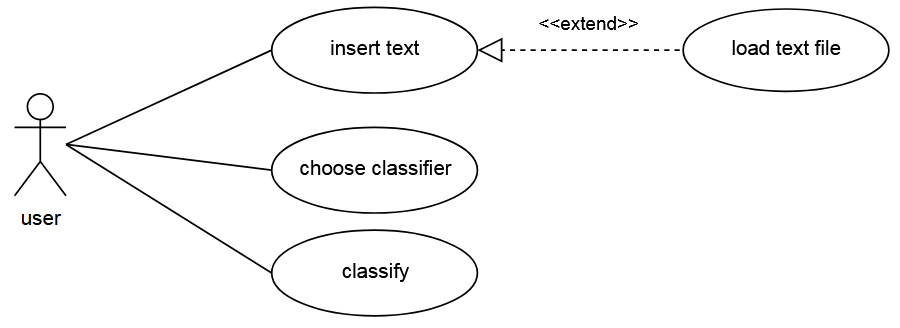
\includegraphics[width=0.8\linewidth]{images/use-case-diagram.png}
	\caption{%
		مخطط حالات الاستخدام للتطبيق.
	}
	\label{fig:man:use-case}
\end{figure}


\section{واجهة التطبيق ودليل استخدامها}

يبيّن الشكل~\ref{fig:man:gui} الواجهة التخاطبية للتطبيق.
يمكن للمستخدم إدخال نص بشكل مباشر باستخدام لوحة المفاتيح أو تحميل ملف نصي عبر الزر \eng{Load File}.
وبالضغط على الزر \eng{Classify} يظهر التطبيق النتيجة.
قد تستغرق هذه العملية زمن، حوالي 4-12 ثانية، بحسب طول وتعقيد النص المدخل.
ويمكن للمستخدم اختيار مُصنّف من القائمة الموجودة تحت اسم \eng{Classifier} (الزاوية اليمنى من الأسفل).
لمعرفة سبب سماح التطبيق للمستخدم بتحديد المصنّف الذي سيتم استخدامه،
انظر إلى بداية الفقرة~\ref{sec:sys:methedology}.


\begin{figure}[htb]
	\centering
	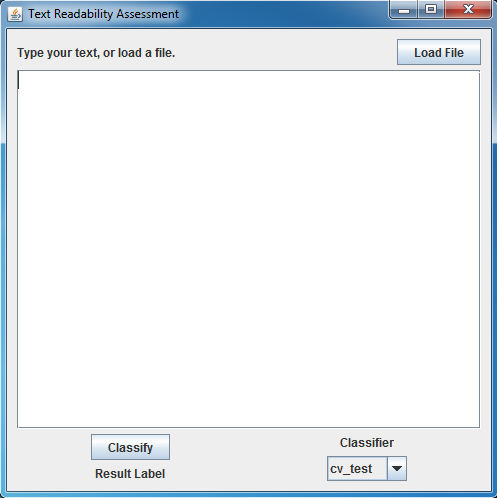
\includegraphics[width=0.7\linewidth]{images/app-gui.png}
	\caption{%
		الواجهة التخاطبية للتطبيق.
	}
	\label{fig:man:gui}
\end{figure}

يبيّن الشكل~\ref{fig:man:ex} مثال على استخدام التطبيق لتقييم مقروئية النص \eng{Amsterdam-int.txt}،
الموجود ضمن مجموعة المعطيات \eng{OSE}.
ونلاحظ أن التطبيق قام بتصنيفه بشكل صحيح كنص متوسط الصعوبة.

\begin{figure}[htb]
	\centering
	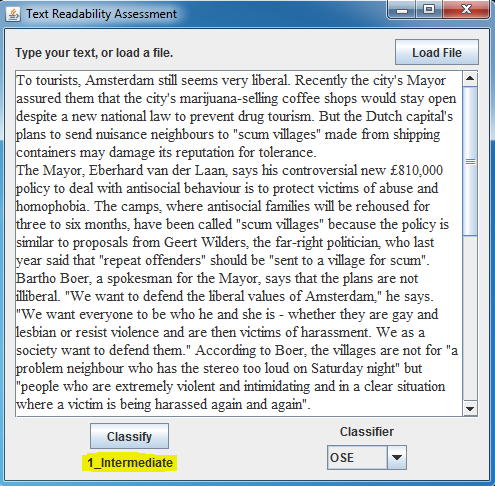
\includegraphics[width=0.7\linewidth]{images/app-ex.png}
	\caption{%
		مثال على استخدام التطبيق.
	}
	\label{fig:man:ex}
\end{figure}

